

\documentclass[11pt]{extarticle}

\usepackage[utf8]{inputenc}
\usepackage{extsizes} % Allow for more sizes such as 14pt or 17pt on document class.
\usepackage{mathtools} % Allows conditional math expressions, etc.

% Don't output references in case they're empty - http://tex.stackexchange.com/questions/74476/how-to-avoid-empty-thebibliography-environment-bibtex-if-there-are-no-refere

\let\myBib\thebibliography
\let\endmyBib\endthebibliography

\renewcommand\thebibliography[1]{\ifx\relax#1\relax\else\myBib{#1}\fi}


\begin{document} 



%% Front page.
\title{06.02 - Machine Learning System Design}

    
    \date{}
    

    

    \maketitle

\newpage
%% Abstract page.


%% Table of contents page.



%% Body start.
\section{Prioritizing what to work on: Spam classification
example}\label{prioritizing-what-to-work-on-spam-classification-example}

If we want to build a spam filter, we first need to know what is the
\emph{x} and the \emph{y} in our problem.

\emph{y} is easy: 1 if spam, 0 if ham.

One way of choosing our \emph{x} features would be to find 100 words
indicative of spam/ham. Then, our feature vector would be full of
boolean features each indicating whether the word appeared in the email
or not.

\subsection{How to spend your time to make it have low
error?}\label{how-to-spend-your-time-to-make-it-have-low-error}

\begin{itemize}
\itemsep1pt\parskip0pt\parsep0pt
\item
  Collect data. Eg ``honeypot'' project.
\item
  Sophisticated features based on email header.
\item
  Sophisticated features based on email body. Eg should ``discount'' and
  ``discounts'' be treated as the same word.
\item
  Develop algorithm to detect misspellings (med1cine, w4tches).
\end{itemize}

\section{Error Analysis}\label{error-analysis}

\subsection{Recommended approach}\label{recommended-approach}

\begin{itemize}
\itemsep1pt\parskip0pt\parsep0pt
\item
  Start with a simple algorithm that you can implement quickly (avoid
  premature optimization).
\item
  Plot learning curves to decide if more data, more features are likely
  to help.
\item
  Error analysis: Manually examnie the examples that your algorithm made
  errors on. See if you spot any trend in the type of examples it is
  making errors on.
\end{itemize}

In the case of the emails, if we have a certain amount of missclassified
emails, we can check the type of them (eg most common are pharma,
replica, steal passwords, \ldots{}) and what features you thjink would
have helped the algorithm to classify them correctly.

Manually doing this can serve the purpose of finding the thing where
spending time is more worth it.

\subsection{The importance of numerical
evaluation}\label{the-importance-of-numerical-evaluation}

It's important to have a reference number (such as accuracy) in order to
know whether doing a change is an improvement or not.

Eg, should discount/discounts/discounted/discounting be treated as the
same word? Check score doing it / not doing it and decide based on that.

\section{Error metrics for skewed
classes}\label{error-metrics-for-skewed-classes}

\subsection{Cancer classification
example}\label{cancer-classification-example}

\begin{itemize}
\itemsep1pt\parskip0pt\parsep0pt
\item
  Logistic regression model.
\item
  1\% Error on test set.
\end{itemize}

Problem: 0.5\% of patients have cancer. An algorithm that simply says
that y = 0 (no cancer) has a 0.5\% of error!!

\textbf{Skewed classes} = when we have a lot more data from a class than
the other one.

\subsection{Different error metrics}\label{different-error-metrics}

In this cases, we need to use different error metrics (confusion
matrix):

\begin{itemize}
\itemsep1pt\parskip0pt\parsep0pt
\item
  Precision: Of all patients where we predicted y = 1, what fraction
  actually has cancer? Equation \ref{eq:precision}.
\item
  Recall: Of all patients that actually have cancer, waht fraction did
  we correctly detect as having cancer? Equation \ref{eq:recall}.
\end{itemize}

\begin{equation} \label{eq:precision}
\text{precision} = \frac{\text{True positives}}{\text{\# predicted positives}}
\end{equation}

\begin{equation} \label{eq:recall}
\text{recall} = \frac{\text{True positives}}{\text{\# actual positives}}
\end{equation}

So, in the case of the model that simply says y = 0, we could use
recall. The result would be a recall of zero, which we will then try to
improve.

\textbf{y = 1} in presence of the most \textbf{rare class}.

\section{Trading Off Precision and
Recall}\label{trading-off-precision-and-recall}

In the example of the cancer algorithm, we want to be very confident as
it's very critical to fail.

Suppose we want to predict y = 1 only if very confident. If we're using
logistic regression, we can simply cut the threshold in which we decide
whether someone has cancer at a higher \%.

Doing that, we get higher precision and lower recall. \bigskip

On the other hand, if we want to avoid mising cases of cancer (avoid
false negatives), we can just cut the threshold lower so more people are
classified as having cancer.

We will have lower precision and higher recall. \bigskip

We can see this in figure \ref{fig:precision_recall_threshold}.

\begin{figure}
\centering
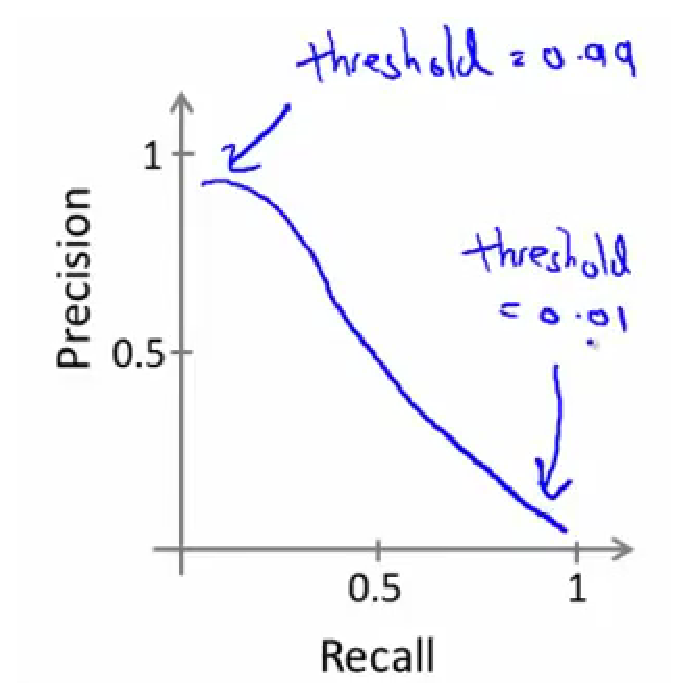
\includegraphics[width=\textwidth]{img/precision_recall_threshold.eps}
\caption{Precision and recall depending on the threshold we cut at.}
\label{fig:precision_recall_threshold}
\end{figure}

\subsection{F score}\label{f-score}

A way to compare precision and recall, as given in equation
\ref{eq:f_score}.

\begin{equation} \label{eq:f_score}
\text{f score} = 2 \frac{PR}{P+R}
\end{equation}

\section{Data For Machine Learning}\label{data-for-machine-learning}

\begin{quote}
It's not the best algorithm that wins, but the one with more data.
\end{quote}

We must make sure the features we have have sufficient info to predict y
accurately, though. A good way to tell that is thinking about whether a
human expert could predict y with the data we have.

\subsection{Large data rationale}\label{large-data-rationale}

Pick an algorithm with many parameters so that it can learn difficult
functions.

Also use a large training set (unlikely to overfit).

Doing this we will have a small train error and the train error will be
more or less equal to the test error. That means that the train error
will be small. That is assuming we have a loooot of data.


%% Body end.

%% Bibliography.

    \nocite{*}

\bibliographystyle{plain}
\bibliography{references}

\end{document}